\documentclass{article}

\usepackage[accepted]{icml2023}

% Packages
\usepackage{graphicx}
\usepackage{booktabs}
\usepackage{multirow}
\usepackage{amsmath, amssymb}
\usepackage{xcolor}
\usepackage{subcaption}
\usepackage{listings}
\usepackage{float}
\usepackage{tcolorbox}
\usepackage{algorithm, algpseudocodex}
\usepackage{epstopdf}
\usepackage[colorlinks=true,
            linkcolor=blue,
            filecolor=blue,
            urlcolor=blue,
            citecolor=blue]{hyperref}

% Graphics
\DeclareGraphicsExtensions{.png,.pdf}

% Aliases
\newcommand{\github}{\href{https://github.com/mikasenghaas/diloco-swarm}{GitHub}}
\newcommand{\wandb}{\href{https://wandb.ai/mikasenghaas/diloco-swarm}{Weights \& Biases}}
\newcommand{\gist}{\href{https://gist.github.com/mikasenghaas/5fa1aa77ea69f187f531a5889983c249}{GitHub Gist}}

% Colors
\definecolor{bblue}{HTML}{5884E2}
\definecolor{oorange}{HTML}{F19E38}
\definecolor{ppurple}{HTML}{9900FF}

% Colored boxes
\newcommand{\orangebox}{\colorbox{oorange!50}{\hspace{0.3em}}}
\newcommand{\bluecircle}{\textcolor{bblue}{\LARGE$\bullet$}}
\newcommand{\purplecircle}{\textcolor{ppurple}{\LARGE$\bullet$}}

% Code
\definecolor{codegreen}{rgb}{0,0.6,0}
\definecolor{codegray}{rgb}{0.5,0.5,0.5}
\definecolor{codepurple}{rgb}{0.58,0,0.82}
\definecolor{backcolour}{rgb}{0.95,0.95,0.95}
\lstdefinestyle{mystyle}{
    backgroundcolor=\color{backcolour},   
    commentstyle=\color{codegreen},
    keywordstyle=\color{magenta},
    numberstyle=\tiny\color{codegray},
    stringstyle=\color{codepurple},
    basicstyle=\ttfamily\footnotesize,
    showspaces=false,                
    showstringspaces=false,
    showtabs=false,                  
    tabsize=2
}
\lstset{style=mystyle}

% Running Title
\icmltitlerunning{DiLoCo-SWARM}

\begin{document}

\begin{titlepage}
\begin{center}
    \Large{\textsc{École Polytechnique Fédérale de Lausanne}}\\
    \vspace{1cm}
    
\includegraphics[width=5cm]{figures/epfl.png}
    \vspace{1cm}
    
    \large{Optional Master Research Project, \textit{January 2025}}\\
    
    \vspace{1cm}
    \rule{\textwidth}{1pt}\vspace{15pt}
    \Huge{DiLoCo-SWARM}
    \rule{\textwidth}{1pt}
    
    \vspace{1cm}
    
    \large{\textsc{Mika Senghaas}\\\texttt{mika.senghaas@epfl.ch}}
    \vspace{\stretch{1}}
    
    \large{
      \textit{Supervisors}\\
      \textsc{Martijn De Vos}, \textsc{Akash Dhasade}, \textsc{Rishi Sharma}}\\
      \vspace{0.5cm}
      \textit{Professor}\\
      \textsc{Anne-Marie Kermarrec}\\
      \vspace{0.5cm}
      \large{\textit{Laboratory}\\
      Scalable Computing Systems (SaCS)\\
    }
\end{center}
\end{titlepage}

% Title
\twocolumn[
  \icmltitle{DiLoCo-SWARM}
  \begin{icmlauthorlist}
    \icmlauthor{Mika Senghaas}{author}
    \icmlauthor{Martijn De Vos}{supervisor}
    \icmlauthor{Akash Dhasad}{supervisor}
    \icmlauthor{Rishi Sharma}{supervisor}
  \end{icmlauthorlist}
  \icmlaffiliation{author}{Author}
  \icmlaffiliation{supervisor}{Supervisor}
  \icmlcorrespondingauthor{Mika Senghaas}{mika.senghaas@epfl.ch}
  \icmlkeywords{Distributed Training, Decentralized AI, SWARM, DiLoCo}
  \vskip 0.3in
]
\printAffiliationsAndNotice{}

% Abstract
\begin{abstract}
  This work proposes \textit{DiLoCo-SWARM}, a decentralized training method that integrates infrequent gradient synchronization from DiLoCo into SWARM's fault-tolerant data-pipeline parallelism. Our experiments show that DiLoCo-SWARM matches the generalization performance of traditional SWARM while reducing synchronization frequency by up to 50x. We further demonstrate that DiLoCo-SWARM scales efficiently to larger models, with communication savings increasing as model size grows.
\end{abstract}

\section{Introduction}

Modern foundation models contain billions of parameters and are trained on trillions of tokens~\cite{chowdhery2022palm,brown2023gpt3,dubey2024llama3,google2024gemini}. Achieving this scale necessitates orchestrating thousands of GPUs to distribute computation~\cite{dubey2024llama3,deepseekai2024}. However, conventional parallelization techniques rely heavily on high-bandwidth interconnects to avoid communication bottlenecks. As a result, cutting-edge models are primarily trained in high-performance clusters (HPCs). Operating these clusters incurs significant costs, thereby restricting research abilities on foundation models to a select group of corporate and state actors~\cite{jaghouar2024intellect1}.

Decentralized training has emerged as a promising alternative. By leveraging low-cost, globally distributed compute resources, decentralized training promises to democratize access to model development. However, this paradigm shift introduces substantial technical challenges, particularly in accommodating latency and bandwidth limitations in Internet connections, heterogeneous compute environments and dynamic node participation.

While decentralized training efforts cannot yet match the 
scale and efficiency of centralized training, the field 
has made significant progress in recent years. INTELLECT-1~\cite{jaghouar2024intellect1}, a 10B parameter model trained collaboratively across the globe, demonstrates this most recently. The model builds on DiLoCo~\cite{douillard2023diloco}, a data parallel method that reduces communication overhead by synchronizing gradients infrequently through a dual optimization scheme. DiLoCo achieves competitive performance with traditional data parallelization but only synchronizes gradients every 500 steps instead of after each step. However, DiLoCo requires each node to store a full model replica, limiting participation to high-performance hardware.

SWARM~\cite{ryabinin2023swarm} offers a promising, though less explored, alternative for larger-scale decentralized training. SWARM combines both data and pipeline parallelism and introduces several novel techniques to enable fault-tolerant training in heterogeneous compute and network conditions. By partitioning the model across nodes, SWARM can train larger models and allow devices with limited resources to participate. However, in its original formulation, SWARM requires frequent gradient synchronization within pipeline stages. 

This work proposes \textit{DiLoCo-SWARM}, a novel approach that integrates DiLoCo-style infrequent gradient synchronization into SWARM parallelism. Our experimental results are summarized in the following contributions:

\begin{enumerate}
  \item \textbf{Convergence.} We demonstrate that SWARM parallelism can effectively integrate DiLoCo and achieve comparable validation perplexity to a synchronous SWARM baseline, while requiring significantly 50x fewer gradient updates.
  \item \textbf{Communication Efficiency.} We show that DiLoCo-SWARM achieves increasing communication savings over SWARM as the model size grows.
  \item \textbf{Robustness.} We validate the robustness of DiLoCo-SWARM to synchronization frequency, and model sizes, underlining its robustness at scale.
\end{enumerate}

We open-source the experiment code and results on \github{} and \wandb{}, along with a distilled version of the training logic in a \gist{} with only a few hundred lines of PyTorch code. We aim for these resources to foster further open-source research on scaling DiLoCo-SWARM parallelism to production-grade systems, following the trajectory of DiLoCo's development.

\section{Background}

This section outlines the foundations of distributed and decentralized learning, detailing core parallelization techniques, key challenges, and recent solutions, with a focus on the DiLoCo and SWARM methods that underpin our proposed approach.

\subsection{Distributed Training}

In distributed training, $n$ nodes collaboratively train a \textit{model} $f_{\theta}$ parameterized by weights $\theta$, on a \textit{dataset} of samples $D = \{(\mathbf{x}_1, \mathbf{y}_1),\dots\}$. This collaboration requires periodic communication of intermediate results between nodes. We will describe two fundamental parallelization techniques relevant to DiLoCo-SWARM.

\begin{figure}[ht]
    \centering
    \begin{subfigure}[b]{0.48\textwidth}
        \centering
        \vspace{0.5cm}
        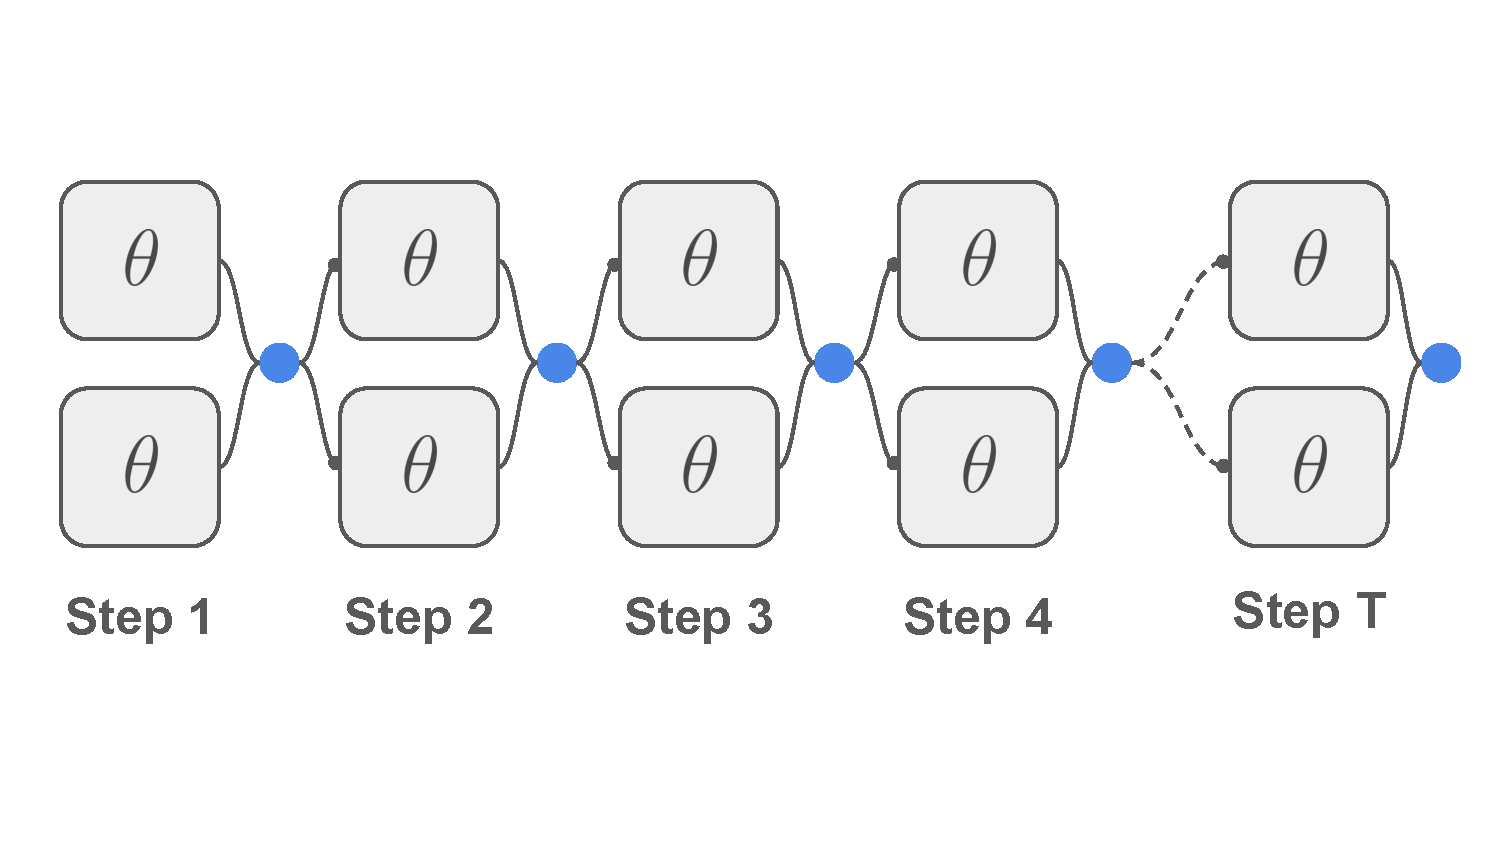
\includegraphics[width=\textwidth]{figures/dp.pdf}
        \caption{\textbf{DP Communication}. Nodes synchronize gradients (\bluecircle) at each step within a DP group.}
        \label{fig:dp}
    \end{subfigure}
    \hfill
    \begin{subfigure}[b]{0.45\textwidth}
        \centering
        \vspace{0.5cm}
        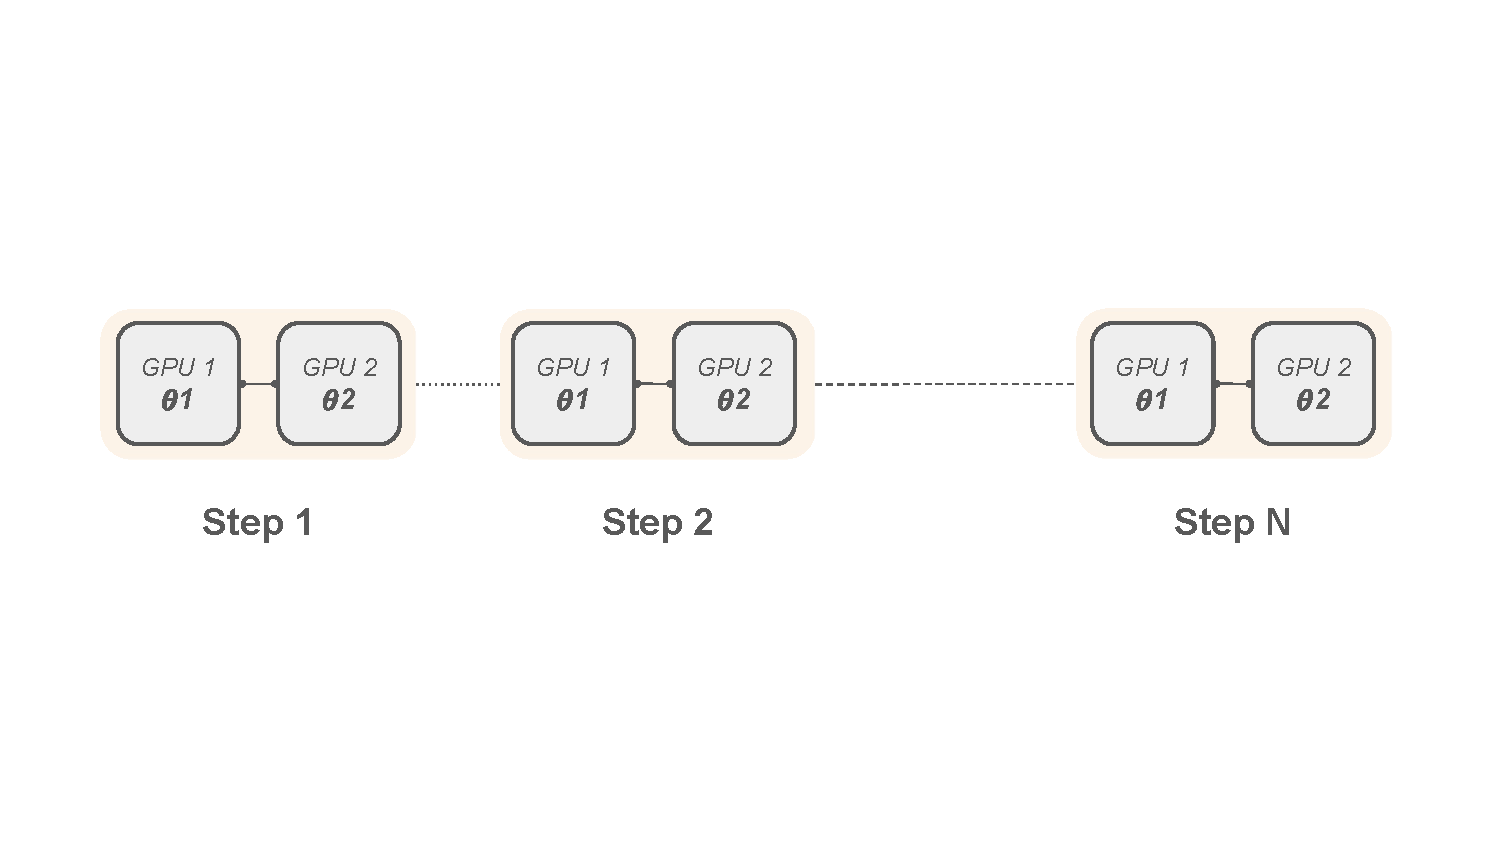
\includegraphics[width=\textwidth]{figures/pp.pdf}
        \caption{\textbf{PP Communication}. Nodes communicate activations and gradients (\orangebox) between adjacent stages within a PP group.}
        \label{fig:pp}
    \end{subfigure}
    \caption{\textbf{DP and PP.} Illustration of communication patterns for $n=2$ DP and PP groups over $T$ training steps. Nodes are represented as boxes, and communication as solid lines. The dotted lines indicate no communication.}
\end{figure}

In \textit{Data Parallelism} (DP)~\cite{dean2012dp}, the dataset is partitioned into $n$ shards, with each node holding a unique shard $D_i$ and a complete model replica $\theta$. Training proceeds as follows: Each node samples a batch from its local data shard, and computes local gradients through a forward and backward pass. Before updating the model, nodes synchronize gradients to ensure identical updates across all nodes (Algorithm~\ref{alg:dp}). Typically, the synchronization is performed using an \texttt{AllReduce} operation. Figure~\ref{fig:dp} illustrates this communication pattern unrolled over $T$ training steps.

\begin{algorithm}
\caption{Data Parallel Gradient Synchronization}
\label{alg:dp}
\begin{algorithmic}[1]
\State {\bfseries Input:} Local Dataset $D_i$, Model $\theta^{(t-1)}$, Optimizer $\mathtt{OPT}$, Loss $\mathcal{L}$
\State Sample batch: $x_i\sim D_i$
\State Compute gradient: $g_i \gets \nabla_{\theta^{(t-1)}} \mathcal{L}(x_i; \theta^{(t-1)})$
\State Sync gradients: $g \gets \frac{1}{n}\sum_{i}^n g_i$ \Comment{$\mathtt{AllReduce}$}
\State Update model: $\theta^{(t)} \gets \mathtt{OPT}(\theta^{(t-1)}, g)$
\end{algorithmic}
\end{algorithm}

In \textit{Pipeline Parallelism} (PP)~\cite{huang2019gpipe}, the model is partitioned into $n$ stages, with each stage holding a unique subset of parameters $\theta_i$. The full model is then represented as a pipeline, where each stage processes a portion of the input sequentially. Communication occurs in two phases during training: activations are sent forward through the pipeline during the forward pass, and gradients are sent backward during the backward pass (Figure~\ref{fig:pp}). Importantly, PP relies solely on point-to-point communication between adjacent stages without all-to-all synchronization.

Despite its simplicity, PP is challenging to optimize in practice due to synchronization delays that cause GPU idle time. For example, the first stage must wait for the full forward and backward pass through the entire pipeline before it can process the next input. Efficient PP implementations, therefore, rely on techniques such as micro-batching and advanced scheduling to minimize idle time and maximize throughput~\cite{harlap2018pipedream, huang2019gpipe}. Further, for large models, the computation-to-communication ratio grows in favor of PP communication, allowing to "hide" communication latency behind computation~\cite{fernandez2024scalingtrends}.

Both parallelization techniques may be combined. We will refer to this form of hybrid parallelism as \textit{Data-Pipeline Parallelism (DPP)}. In this approach, both the dataset and model are partitioned into $\{D_i\}_{i \in [m]}$ and $\{\theta_j\}_{j \in [n]}$, resulting in a two-dimensional grid of $m \times n$ nodes, where the $(i,j)$-th node is responsible for data shard $D_i$ and model shard $\theta_j$. Figure~\ref{fig:dpp} illustrates the communication pattern for a $2\times 2$ DPP system. PP and DP communication is interleaved: First, nodes within each PP group communicate activations and gradients to accumulate local gradients independently. Then, nodes synchronize local gradients within each DP group before updating their model shard.

\begin{figure}[ht]
    \centering
    \vspace{0.5cm}
    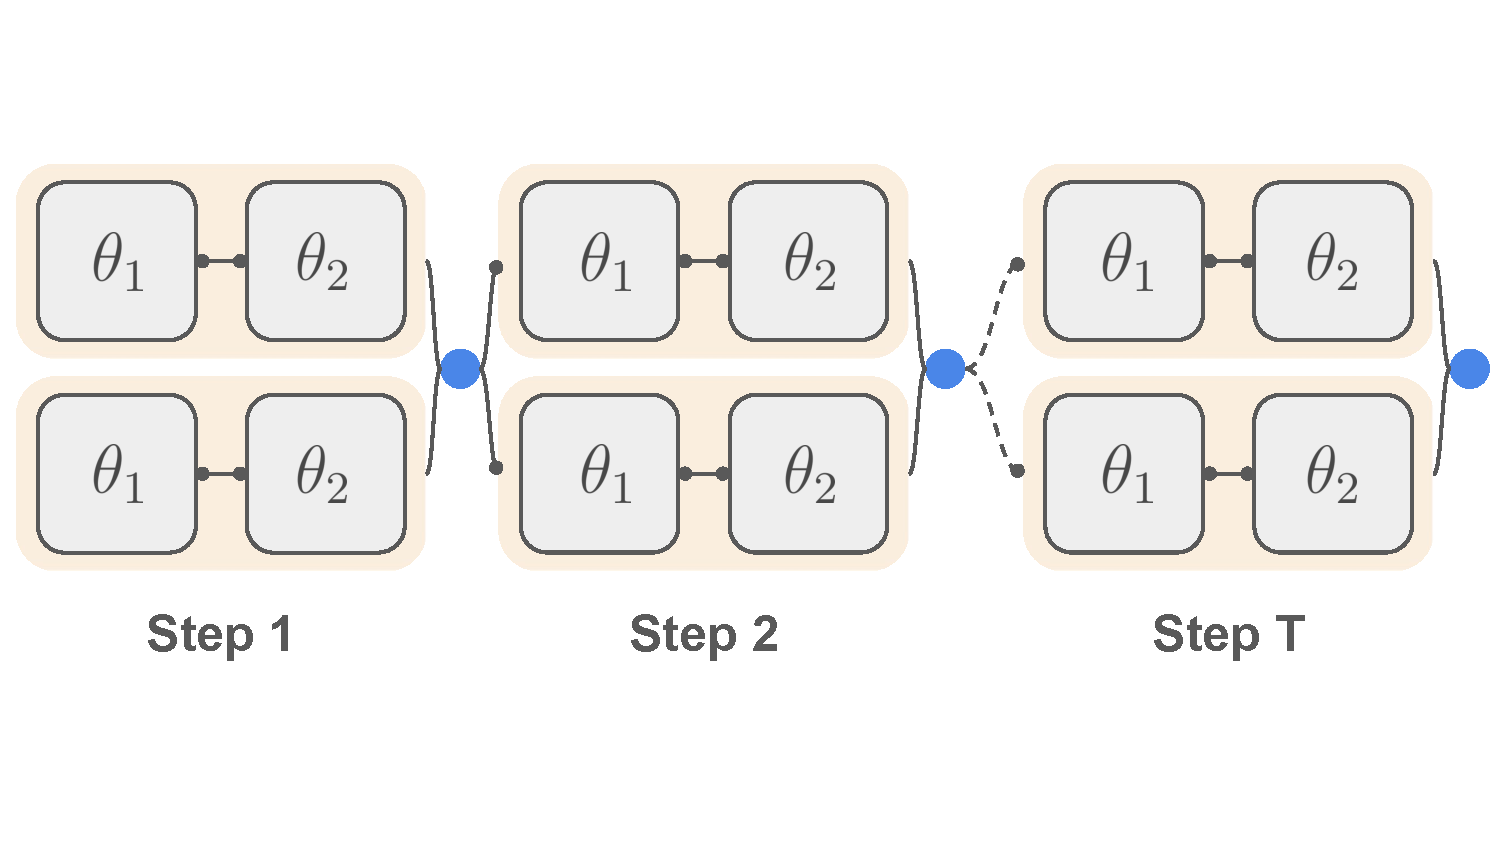
\includegraphics[width=0.48\textwidth]{figures/dpp.pdf}
    \caption{\textbf{DPP.} Illustration of communication patterns in a hybrid parallelism (DPP) setup with a $2 \times 2$ grid of nodes. PP and DP communication are interleaved: PP groups accumulate local gradients independently (\orangebox). Then, DP groups synchronize gradients before updating the model (\bluecircle).}
    \label{fig:dpp}
\end{figure}

All described parallelization techniques produce equivalent gradient updates and converge to identical model parameters $\theta^{(t)}$. However, they differ fundamentally in how computation and communication are distributed, which impacts efficiency depending on model size, hardware, and network configuration~\cite{hagemann2024parallelization, fernandez2024scalingtrends}.

\subsection{Decentralized Learning}

Decentralized learning builds on foundational work in federated learning (FL)~\cite{mcmahan2016fl}, which enables learning on a network
of mobile devices that retain private access to their own data and periodically share local model updates with a central server for aggregation~\cite{mcmahan2016fl,wang2020fedma}. More recently, decentralized learning has shifted toward large-scale training on preemptible, low-cost hardware, often referred to as \textit{volunteer computing}. While many FL concepts remain relevant, modern research in decentralized learning focuses on improving training efficiency under the unique constraints of decentralized environments: orders-of-magnitude slower interconnect, network and device heterogeneity, and instances joining and leaving training at any time.

Recent research addresses all of these challenges: \citeauthor{zhang2020volatileinstances} first explored fault-tolerant training on pre-emptible instances, which SWARM extended to support hybrid parallelism in heterogeneous environments~\cite{ryabinin2023swarm}. Another key area of research concerns reducing the communication volume of decentralized training to combat the slow interconnect. DiLoCo~\cite{douillard2023diloco} reduces the gradient synchronization frequency via a dual optimization scheme, while DeMo~\cite{peng2024demo} synchronizes only fast-moving momentum components. SPARTA~\cite{exo2025sparta} proposes to only communicate a small random subset of gradients at each step.

Efforts to scale decentralized training to production systems are ongoing. Notable examples include collaborative training platforms such as Transformers Together~\cite{diskin2021collaborativelearning} and Petals~\cite{borzunov2023petals}, which enable distributed inference for large language models. The recent INTELLECT-1 run~\cite{jaghouar2024intellect1} demonstrated the feasibility of decentralized training at scale by collaboratively training a 10-billion-parameter model across the globe.

\subsection{DiLoCo}

In decentralized training, synchronizing gradients at every step, as in traditional DP (Algorithm~\ref{alg:dp}), can be prohibitive due to slow interconnects. DiLoCo~\cite{douillard2023diloco} addresses this limitation by reducing synchronization frequency through a local-global optimization scheme, shown in Algorithm~\ref{alg:diloco}. Each node trains locally for a fixed number of steps, $H$, using a local optimizer. After $H$ steps, nodes compute their pseudo-gradient (the difference between the initial and updated parameters) and synchronize it using a global optimizer to update a shared model.

\begin{algorithm}
\caption{DiLoCo Gradient Synchronization}
\label{alg:diloco}
\begin{algorithmic}
\State \textbf{Input:} Local dataset $D_i$, Model $\theta^{(t-1)}$, Optimizers $\mathtt{OPT}_L$, $\mathtt{OPT}_G$, Loss $\mathcal{L}$, Num. Local Steps $H$ 
\State Copy global model: $\theta_i^{(t-1)} \gets \theta^{(t-1)}$
\For{$H$ steps}
  \State Sample batch: $x \sim D_i$
  \State Compute gradient: $g_i \gets \nabla_{\theta_i} \mathcal{L}(x_i; \theta_i^{(t-1)})$
  \State Update local model: $\theta_i^{(t-1)} \gets \mathtt{OPT}_L(\theta_i^{(t-1)}, g_i)$
\EndFor
\State Compute pseudo-gradient: $\Delta_i \gets \theta_i^{(t-1)} - \theta^{(t-1)}$
\State Sync pseudo-gradients: $\Delta \gets \frac{1}{n} \sum_{i=1}^n \Delta_i$ \Comment{$\mathtt{AllReduce}$}
\State Update global model: $\theta^{(t)} \gets \mathtt{OPT}_G(\theta^{(t-1)}, \Delta)$
\end{algorithmic}
\end{algorithm}

Figure~\ref{fig:diloco} illustrates the communication pattern of DiLoCo in contrast to DP (Figure~\ref{fig:dp}). Nodes only synchronize pseudo-gradients every $H$ steps, thus reducing communication costs by $1/H$. Empirical results show that DiLoCo with $H=500$ matches the generalization performance of a synchronous DP baseline while reducing communication by a factor of 500~\cite{douillard2023diloco,jaghouar2024opendiloco}. However, like DP, DiLoCo is limited by the memory capacity of individual nodes, making it unsuitable for models that exceed local memory. Scaling DiLoCo requires techniques such as gradient quantization~\cite{jaghouar2024intellect1} or parameter offloading~\cite{cui2016}.

\begin{figure}[ht]
    \centering
    \vspace{0.5cm}
    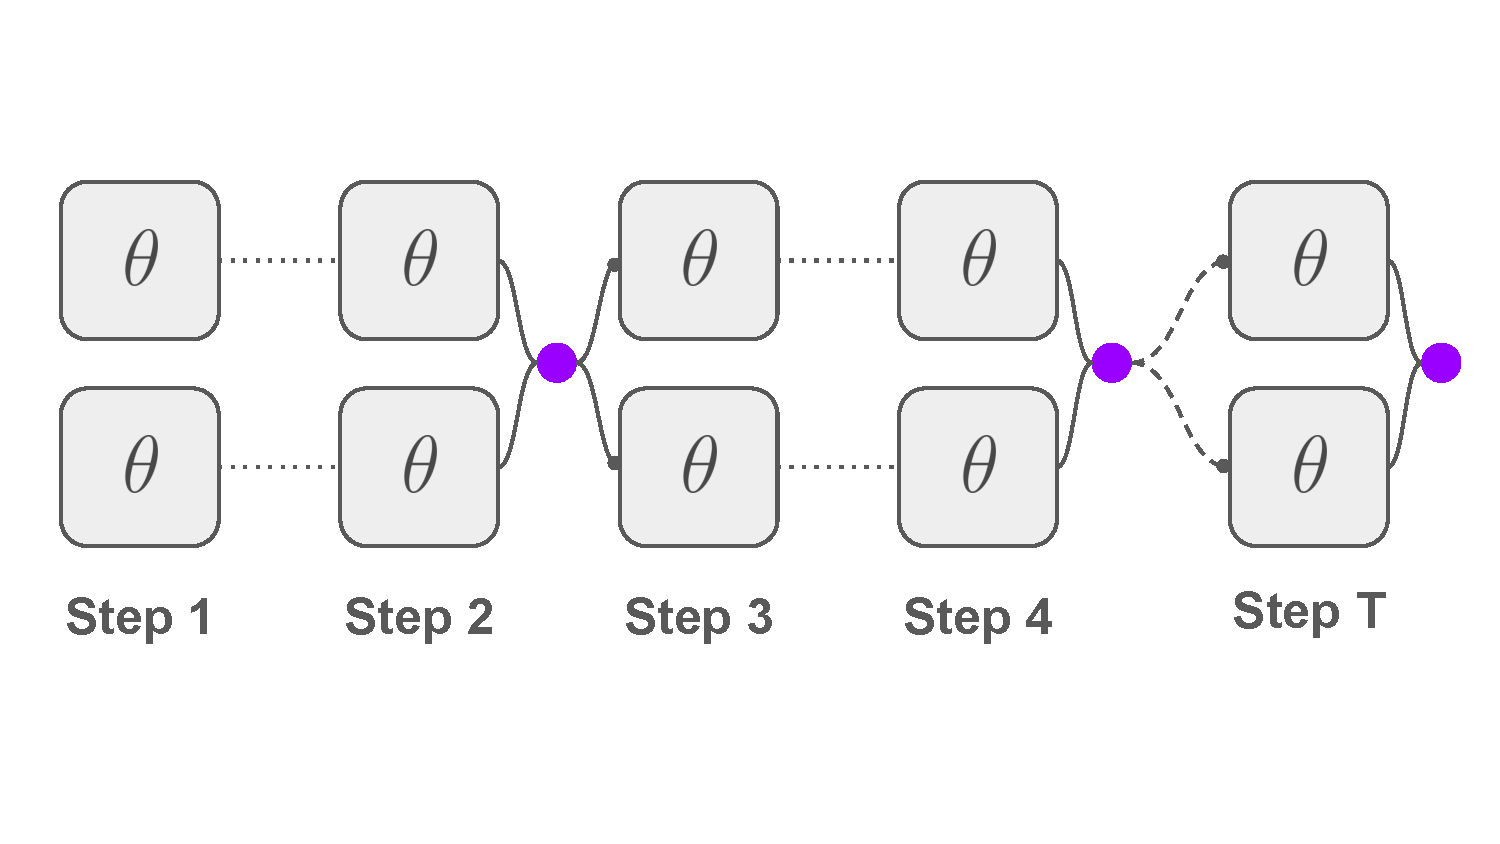
\includegraphics[width=0.45\textwidth]{figures/diloco.pdf}
    \caption{\textbf{DiLoCo.} Comparison of communication patterns for a $n=2$ DiLoCo group over $T$ training steps. Unlike traditional DP, DiLoCo synchronizes pseudo-gradients (\purplecircle) every $H=2$ steps, reducing total communication by a factor of $1/2$.}
    \label{fig:diloco}
\end{figure}

\subsection{SWARM}

While DiLoCo reduces communication frequency, it does not address memory limitations. Sharding the model across nodes, as in pipeline parallelism (PP), is a natural solution. However, traditional PP is poorly suited to decentralized environments due to its sequential nature, which causes significant idle time when nodes have heterogeneous performance. Additionally, a single node failure can stall the entire pipeline.

SWARM parallelism~\cite{ryabinin2023swarm} addresses these limitations by introducing a fault-tolerant data-pipeline parallelism (DPP) approach. Rather than relying on a fixed grid of nodes, SWARM constructs stochastic pipelines dynamically. During the forward pass, each node forwards activations to a randomly selected peer in the next stage, with probability proportional to the peer's throughput. The backward pass follows the same path in reverse to ensure gradient consistency. Once all micro-batches are processed, nodes within each stage form DP groups and synchronize local gradients before updating the model.

This \textit{stochastic wiring} approach has two key advantages: (1) it naturally balances workloads in heterogeneous environments by routing activations to faster nodes, and (2) it enables the pipeline to recover from node failures by re-routing activations or gradients to available nodes. As long as each stage has at least one active node, SWARM remains functional.

A key insight of SWARM is the so-called \textit{Square-Cube Law}~\cite{ryabinin2023swarm}, which states that the communication cost of pipeline parallelism grows quadratically while the computation cost grows cubically for increasing model sizes. Hence, nodes spend more time computing than communicating in large models, allowing them to hide the communication latency behind computation. This leads to the unintuitive consequence that larger models become more communication-efficient.

\begin{figure}[ht]
    \centering
    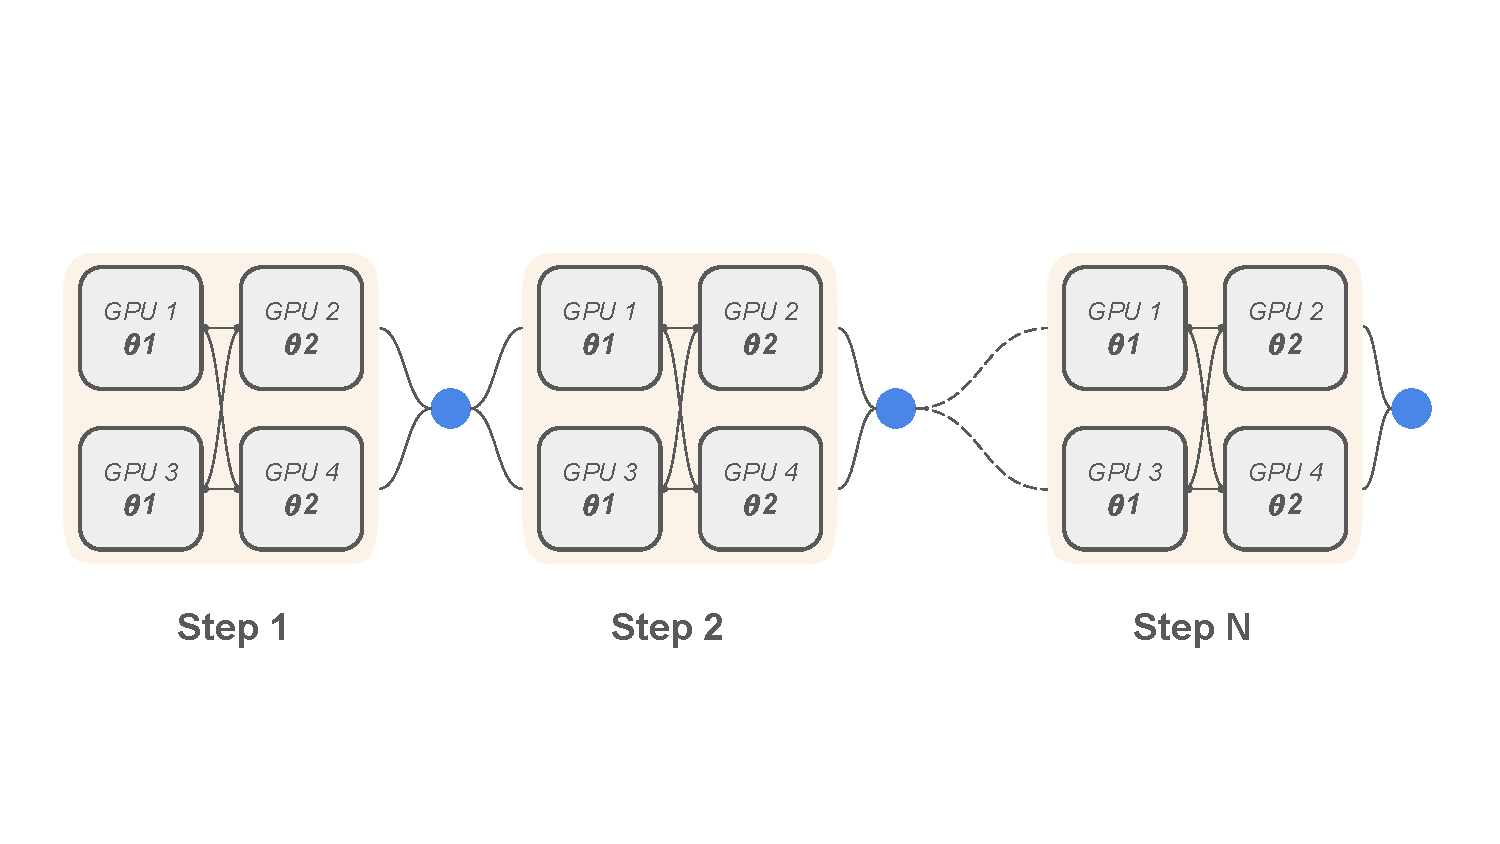
\includegraphics[width=0.45\textwidth]{figures/swarm.pdf}
    \caption{\textbf{SWARM.} Illustration of communication in a $2 \times 2$ SWARM. As in DPP, PP (\orangebox) and DP (\bluecircle) communication is interleaved. Crucially, any node may communicate with any other node in adjacent stages, increasing fault-tolerance and throughput in heterogeneous environments.}
    \label{fig:swarm}
\end{figure}

\section{DiLoCo-SWARM}

SWARM enables large-scale, fault-tolerant data-pipeline parallel (DPP) training in decentralized settings by dynamically constructing stochastic pipelines. However, its data-parallel component still requires frequent gradient synchronization, resulting in high communication costs. In contrast, DiLoCo~\cite{douillard2023diloco} reduces synchronization frequency through local-global optimization but is limited by memory constraints in large models.

This motivates \textit{DiLoCo-SWARM}, a decentralized training method that combines the communication efficiency of DiLoCo with the scalability and fault-tolerance of SWARM. By replacing SWARM's data-parallel groups with DiLoCo groups, DiLoCo-SWARM significantly reduces the frequency of costly
all-to-all gradient synchronization within SWARM stages (Figure~\ref{fig:diloco-swarm}).

\begin{figure}[ht]
    \centering
    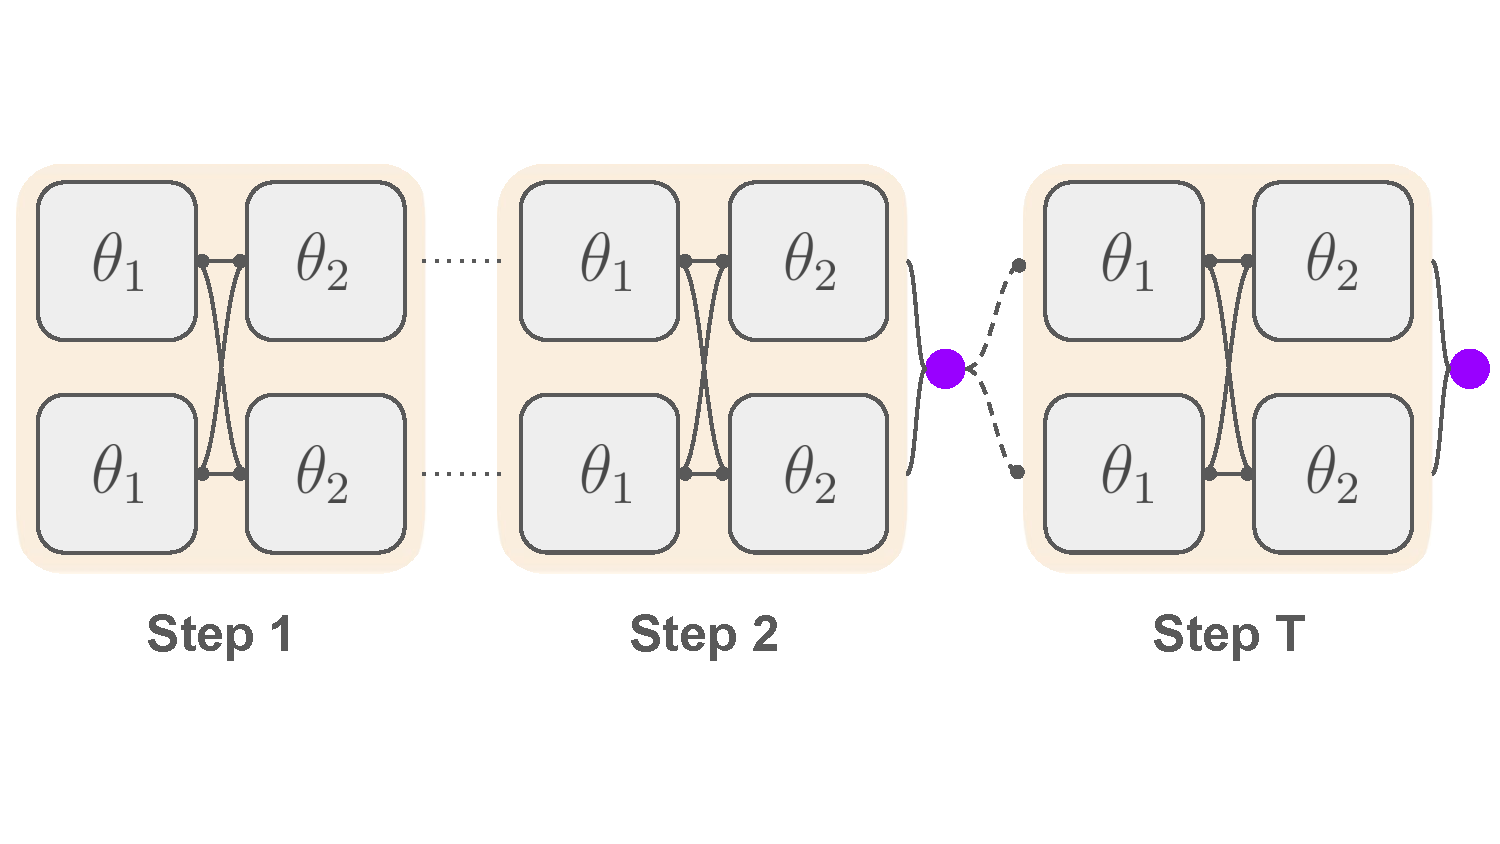
\includegraphics[width=0.45\textwidth]{figures/diloco-swarm.pdf}
    \caption{\textbf{DiLoCo-SWARM.} The communication patterns of DiLoCo-SWARM for $4$ nodes in a $2\times 2$ grid. DiLoCo-SWARM replaces SWARM's frequent gradient synchronization with less frequent DiLoCo-style synchronization of pseudo-gradients (\purplecircle).}
    \label{fig:diloco-swarm}
\end{figure}

\subsection{Algorithm}

Algorithm~\ref{alg:diloco-swarm} describes the algorithmic details of DiLoCo-SWARM. For simplicity, we assume a grid of $m \times n$ nodes, though the method generalizes to any number of nodes per stage. 

Each node begins with a copy of the global model shard $\theta_j^{(t-1)}$. During the inner optimization loop, nodes perform $H$ local steps, stochastically forwarding activations and gradients to adjacent stages and updating their local model shard $\theta_{i,j}$ using a local optimizer. After $H$ steps, nodes compute pseudo-gradients $\Delta_{i,j}$ and synchronize within their stage to update the global model shard $\theta_j^{(t)}$ using a global optimizer.

DiLoCo-SWARM combines SWARM's stochastic wiring during local steps with DiLoCo to synchronize within SWARM stages. In doing so, the method reduces the points
of gradient synchronization, resulting in more communication-efficient training. Unlike DiLoCo, which cuts communication by a factor of $H$, DiLoCo-SWARM cuts communication by a factor of $H$ times the fraction of the total communication cost incurred by gradient synchronization. Furthermore, due to stochastic wiring, gradients may depend on batches sampled from different data shards, resulting in data mixing across nodes.

\begin{algorithm}
\caption{DiLoCo-SWARM}
\label{alg:diloco-swarm}
\begin{algorithmic}[1]
\State \textbf{Input:} Data shard $D_i$, Model shard $f^{(j)}$, Global model shard parameters $\theta_{j}^{(t-1)}$, Loss $\mathcal{L}$, Optimizers $\mathtt{OPT}_{L}$ and $\mathtt{OPT}_{G}$, Local Steps $H$
\Procedure{FwdBwd}{}
  \If{$j = 1$} \Comment{First stage}
    \State Sample batch: $x_i \sim D_i$
    \State Forward: $a_{ij} \gets f^{(j)}_{\theta_{ij}}(x_i)$
    \State Send forward: $\mathtt{send}(a_{ij}, j+1)$ 
    \State Receive backward: $g_{i,j+1} \gets \mathtt{recv}(j+1)$
    \State Compute gradient: $g_{ij} \gets g_{i,j+1} \cdot \nabla_{\theta_{ij}} f^{(j)}_{\theta_{ij}}(a_{ij})$
  \ElsIf{$j = n$} \Comment{Last stage}
    \State Receive forward: $a_{i,j-1} \gets \mathtt{recv}(j-1)$
    \State Forward: $a_{ij} \gets f^{(j)}_{\theta_{ij}}(a_{i,j-1})$
    \State Compute gradient: $g_{ij} \gets \nabla_{\theta_{ij}} \mathcal{L}(a_{ij})$
    \State Send backward: $\mathtt{send}(g_{ij}, j-1)$
  \Else \Comment{Intermediate stages}
    \State Receive forward: $a_{ij-1} \gets \mathtt{recv}(j-1)$
    \State Forward: $a_{ij} \gets f^{(j)}_{\theta_{ij}}(a_{i,j-1})$
    \State Send forward: $\mathtt{send}(a_{ij}, j+1)$
    \State Receive backward: $g_{i,j+1} \gets \mathtt{recv}(j+1)$
    \State Compute gradient: $g_{ij} \gets g_{i,j+1} \cdot \nabla_{\theta_{ij}} f^{(j)}_{\theta_{ij}}(a_{ij})$
    \State Send backward: $\mathtt{send}(g_{ij}, j-1)$
  \EndIf
  \Return $g_{ij}$
\EndProcedure
\State Copy global model: $\theta_{ij}^{(t-1)} \gets \theta_j^{(t-1)}$
\For{$H$ steps}
  \State Compute gradients: $g_{i,j} \gets \mathtt{FwdBwd}()$
  \State Update local model: $\theta_{ij}^{(t-1)} \gets \mathtt{OPT}_{L}(\theta_{ij}^{(t-1)}, g_{i,j})$
\EndFor
\State Compute pseudo-gradient: $\Delta_{i,j} \gets \theta_{ij}^{(t-1)} - \theta_j^{(t-1)}$
\State Sync pseudo-gradients: $\Delta_j \gets \frac{1}{m}\sum_i^m \Delta_{i,j}$
\State Update global model: $\theta_j^{(t)} \gets \mathtt{OPT}_{G}(\theta_j^{(t-1)}, \Delta_j)$
\end{algorithmic}
\begin{minipage}{\linewidth}
\vspace{1.5ex}
\small
\textbf{Note:} The \texttt{recv} and \texttt{send} functions perform many-to-one and one-to-many communication with adjacent stages using
stochastic wiring. Details are abstracted away for brevity.
\end{minipage}
\end{algorithm}

\subsection{Implementation}

We release a complete implementation of the proposed method, along with a distilled, single-file training script that supports DP, PP, DPP, SWARM, and DiLoCo-SWARM. The implementation is designed for simplicity, relying solely on PyTorch's \texttt{torch.distributed} package for communication. 

The training script is minimal, consisting of only a few hundred lines of code, making it an accessible resource for researchers to explore and experiment with various distributed training techniques. It supports emulation of multiple nodes via threading and integrates with HuggingFace for model and dataset loading. 

While the implementation prioritizes readability over efficiency, it provides a foundation for future work on decentralized training systems. Inspired by open-source efforts like NanoGPT~\cite{karpathy2024nanogpt}, we aim to foster further research and experimentation in decentralized learning.

\section{Experiments}

In this section, we validate the effectiveness of DiLoCo-SWARM through a series of experiments on a language modeling task. Our experiments evaluate the impact of DiLoCo-style gradient synchronization within SWARM on convergence, communication cost, and scalability across model sizes. The setup largely follows the experimental protocol of DiLoCo~\cite{douillard2023diloco}, with adaptations for the SWARM framework.

\subsection{Setup}

We use the FineWeb-Edu dataset~\cite{penedo2024fineweb}, a large pre-training corpus of educational web content, for all experiments. FineWeb-Edu is chosen for its high token efficiency, allowing models to achieve strong performance on downstream benchmarks such as HellaSwag~\cite{zellers2019hellaswag} with significantly less data~\cite{karpathy2024nanogpt}.

We train various sizes of GPT-2 models~\cite{radford2019gpt2}, following the original architecture hyperparameters, as summarized in Table~\ref{tab:models}. To avoid additional gradient communication in pipelined settings, we do not share the weights of the embedding matrix and language modeling head. Unless otherwise stated, we train GPT-2 Small from scratch.

Hyper-parameters are adapted from the tuning done in DiLoCo (Douillard et al., 2023): The default local optimizer is AdamW~\cite{loshchilov2019adamw} with a linearly warmed up learning rate of $4\cdot10^{-4}$, and a weight decay of $0.01$. When DiLoCo is active, we use a Nesterov
with a learning rate of $0.7$ and a momentum of $0.9$ as the global optimizer. A detailed description of the hyperparameters is provided in Table~\ref{tab:hyperparameters} in the Appendix.

Our main evaluation metric is the validation perplexity on a held-out set of 10M tokens from FineWeb-Edu. We evaluate during and after training to show the convergence against the number of training steps, as well as the total communication cost.

All experiments were conducted on a single node with eight co-located H100 GPUs
on \href{https://app.primeintellect.com/}{Prime Intellect Compute}.

\begin{table}[h]
\centering
\begin{tabular}{lcccc}
\toprule
\textbf{Model} & \textbf{Layers} & \textbf{Heads} & \textbf{Hidden Size} & \textbf{Params} \\
\midrule
Tiny & 4 & 4 & 128 & $\sim$14M \\
Small & 12 & 12 & 768 & $\sim$180M \\
Medium & 24 & 16 & 1024 & $\sim$405M \\
Large & 36 & 20 & 1280 & $\sim$800M \\
\bottomrule
\end{tabular}
\caption{\textbf{Model Sizes.} GPT-2 configurations used in experiments. Parameter counts reflect non-shared embedding and head weights.}
\label{tab:models}
\end{table}

\subsection{Main Experiment: DiLoCo-SWARM}

Our main experiment compares DiLoCo-SWARM to two baselines: a single-node setup and a standard SWARM configuration. The weak baseline trains on a single GPU for 2,000 steps, with a batch size of 512 and a sequence length of 1,024, resulting in a data budget of 1B tokens. The strong baseline is a 4x2 SWARM setup (eight workers distributed across two pipeline stages), which performs step-synchronous gradient synchronization. DiLoCo-SWARM follows the same 4x2 setup but replaces step-synchronous gradient synchronization with DiLoCo-style synchronization every 50 steps. This reduces the communication cost within data-parallel groups by a factor of 50.

\begin{figure*}[t]
  \centering
  \begin{subfigure}[b]{0.48\textwidth}
    \centering
    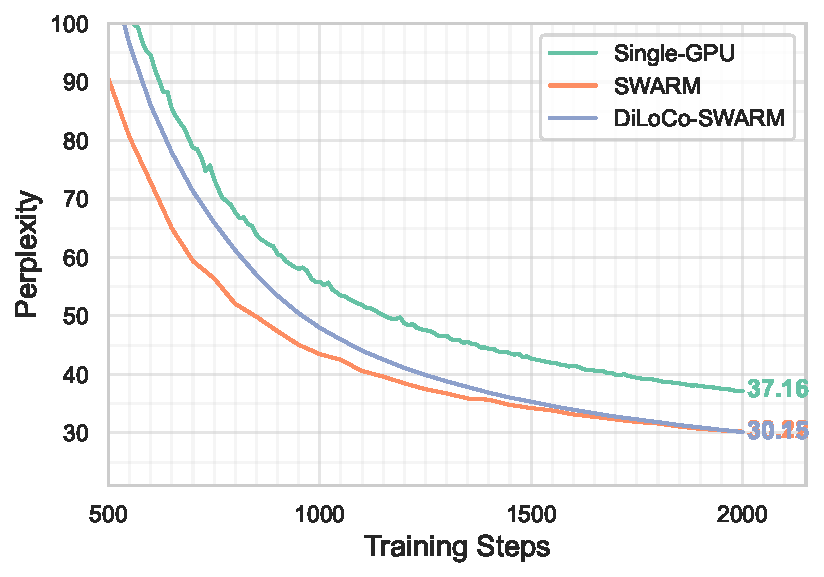
\includegraphics[width=\textwidth]{figures/experiment1-1.pdf}
    \caption{Validation perplexity vs. training steps.}
    \label{fig:experiment1-1}
  \end{subfigure}
  \hfill
  \begin{subfigure}[b]{0.48\textwidth}
    \centering
    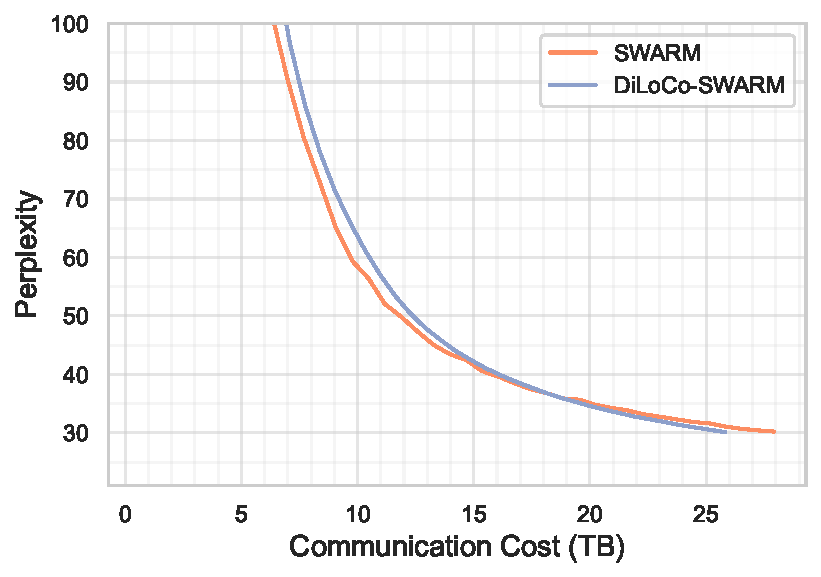
\includegraphics[width=\textwidth]{figures/experiment1-2.pdf}
    \caption{Validation perplexity vs. communication cost.}
    \label{fig:experiment1-2}
  \end{subfigure}
  \caption{\textbf{Main Result.} DiLoCo-SWARM matches the strong baseline in generalization performance, achieving a final validation perplexity of 30.15. Despite synchronizing gradients 50x fewer times, DiLoCo-SWARM incurs only a moderate reduction in total communication cost due to the dominance of pipeline communication in small models.}
  \label{fig:experiment1}
\end{figure*}


Figure~\ref{fig:experiment1-1} shows that DiLoCo-SWARM closely matches the strong SWARM baseline, with a final validation perplexity of 30.15 compared to 30.22. This confirms that infrequent gradient synchronization does not negatively impact convergence.

Figure~\ref{fig:experiment1-2} shows the total communication cost for the same
experiments. Surprisingly, the total communication cost is only moderately reduced in DiLoCo-SWARM compared to SWARM. This finding points at a an important difference between DiLoCo and DiLoCo-SWARM. In DiLoCo, synchronizing gradients every $H$ translates to a proportional reduction in communication cost. DiLoCo-SWARM, in contrast, interleaves DP and PP communication. Since
DiLoCo can only reduce DP communication cost, PP communication cost remains
constant. Figure~\ref{fig:communication-cost-scaling} shows the fraction of the communication cost for 4x2 SWARM training increasingly large models. It illustrates that DP communication cost scales faster and dominates the total communication cost for larger models. This finding suggests that DiLoCo-SWARM is more effective in reducing the communication cost for larger models.

\begin{figure}[ht]
  \centering
  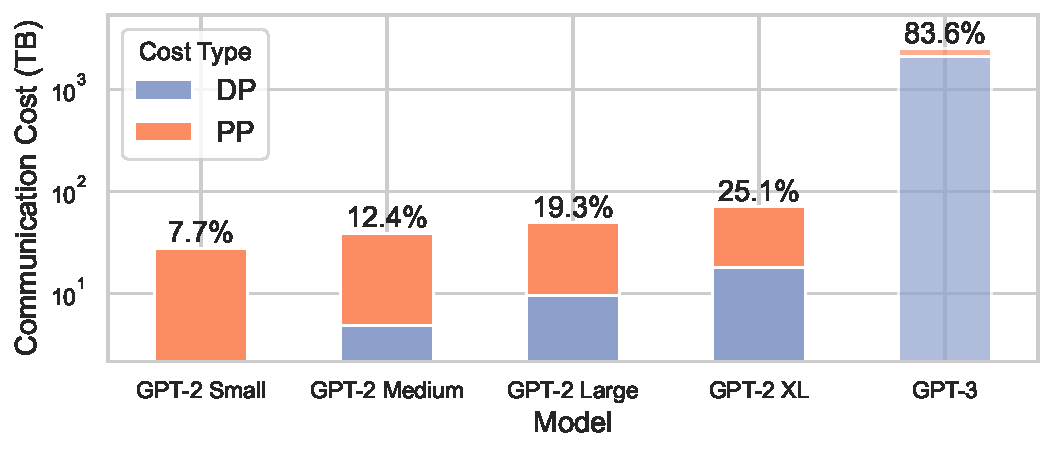
\includegraphics[width=0.45\textwidth]{figures/square-cube-law.pdf}
  \caption{\textbf{Communication Cost Scaling} We show the (log) communication
  cost incurred by DP and PP communication for 4x2 SWARMs in the common training
  setup. Because of the square-cube law, PP communication dominates the total communication for smaller models, but DP communication dominates for larger models.} 
  \label{fig:communication-cost-scaling}
\end{figure}

\subsection{Communication Frequency Ablation}

We investigate the impact of varying the synchronization frequency within pipeline stages on convergence. Specifically, we train five models with synchronization intervals of $\{10, 20, 50, 100, 200\}$ steps, using the same setup as the main experiment.

Table~\ref{tab:experiment2} shows that generalization performance improves with more frequent synchronization. Synchronizing every 10 steps achieves the best validation perplexity of 27.95 but the performance degrades only mildly when decreasing the frequency. A good trade-off between communication efficiency and performance is observed at 50 steps for our training setup. It is worth noting that this is more frequent compared to the 500 steps reported in DiLoCo. We attribute this difference to a significantly larger number of training steps in DiLoCo's setup, allowing for less frequent synchronization. We believe that with more training steps, a similar frequency can be achieved with DiLoCo-SWARM.

\begin{table}[ht]
\centering
\begin{tabular}{lcc}
\toprule
\textbf{Freq. (steps)} & \textbf{Val. PPL} & \textbf{$\Delta$ (Abs./Rel.)} \\ 
\midrule
10 & 27.95 & - \\
20 & 28.61 & +0.66 / +2.36\% \\
50 & 30.15 & +2.20 / +7.87\% \\
100 & 30.49 & +2.54 / +9.09\% \\
200 & 31.27 & +3.32 / +11.88\% \\
\bottomrule
\end{tabular}
\caption{\textbf{Communication Frequency Ablation.} Validation perplexity at different synchronization intervals.}
\label{tab:experiment2}
\end{table}

\subsection{Model Size Ablation}

Finally, we assess the scalability of DiLoCo-SWARM by training four GPT-2 model sizes (Tiny, Small, Medium, and Large) under the same conditions. Figure~\ref{fig:experiment3} shows that DiLoCo-SWARM consistently improves validation perplexity by approximately 18\% over the single-node baseline across all tested model sizes. One noticable outlier is the largest model, which exceeds the single GPU baseline later. We attribute this to untuned hyperparameters, and hypothesize that similar results could be obtained with more tuning. Overall, we conclude that DiLoCo-style gradient synchronization scales effectively with increasing model size.

\begin{figure}[ht]
  \centering
  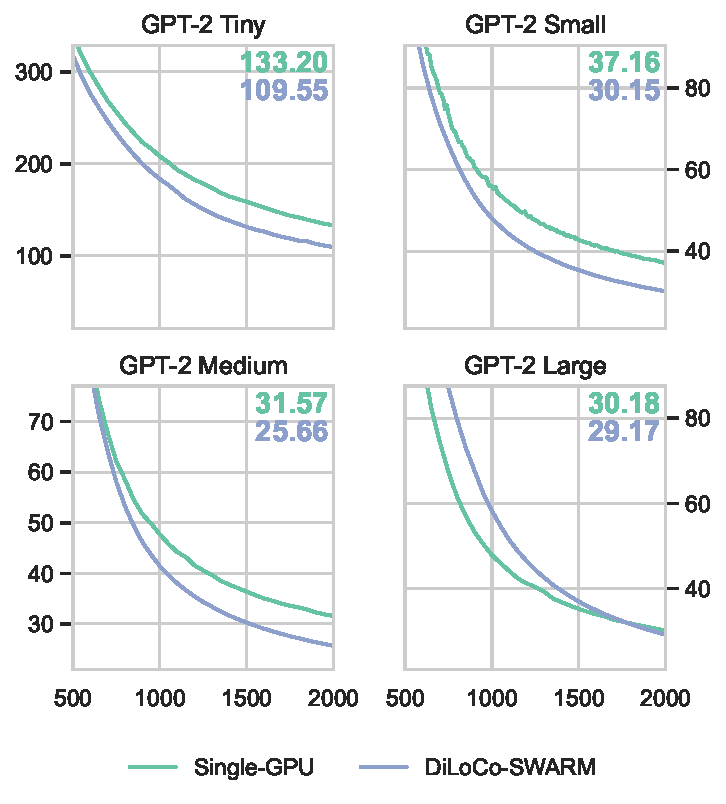
\includegraphics[width=0.48\textwidth]{figures/experiment3.pdf}
  \caption{\textbf{Scalability with Model Size.} DiLoCo-SWARM improves
  generalization performance over the single-node baseline across different
  GPT-2 model sizes.}
  \label{fig:experiment3}
\end{figure}

\section{Conclusion}

In this work, we introduced DiLoCo-SWARM, a decentralized training method that combines the communication efficiency of gradient synchronization of DiLoCo with the scalability and fault-tolerance of SWARM parallelism. By combining both methods, DiLoCo-SWARM reduces communication costs without compromising convergence performance.

Our experimental results on language modeling tasks using the GPT-2 family of models demonstrate that DiLoCo-SWARM matches the generalization performance of traditional SWARM while reducing gradient synchronization frequency by up to 50x. The method shows stronger communication savings for larger models, where data-parallel communication becomes the dominant cost. These findings suggest that DiLoCo-style synchronization is compatible with SWARM and can be a practical solution for scaling decentralized training to larger models.

\section{Future Work}

While this work demonstrates the feasibility of DiLoCo-SWARM, several limitations remain, suggesting directions for future research.

\subsection{Hyperparameter Tuning}

Our experiments assumed that the hyperparameters from DiLoCo~\cite{douillard2023diloco} directly apply to DiLoCo-SWARM. While these hyperparameters provide a reasonable starting point, they may not be optimal for the different dataset, model architecture, and training setup used in this work. Future research should include a thorough hyperparameter sweep, focusing on key parameters such as batch size, learning rates, and learning rate schedules. Given the compute budget constraints, hyperparameter tuning should first be conducted on smaller models and then extrapolated to larger scales.

\subsection{Training Duration}

The experiments in this work were conducted on the GPT-2 family of models, which are small by today's standards. Additionally, models were trained on less than 10 billion tokens, meaning they were still in the early stages of training. In contrast, prior DiLoCo and SWARM experiments trained models on over 50 billion tokens, requiring multiple days of GPU time. To obtain more robust results on late-stage training performance, future experiments should consider increasing the data budget and training duration.

\subsection{Decentralized Setting}

All experiments were conducted on co-located GPUs with fast and reliable interconnectivity. However, one of the primary motivators for SWARM is to enable decentralized training across heterogeneous and unreliable hardware with slower network connections. While our findings suggest that DiLoCo-style gradient synchronization is compatible with SWARM, they remain to be validated in a truly decentralized setting with more pipeline stages and nodes per stage. Future work should explore DiLoCo-SWARM in real-world decentralized environments. This likely requires further optimizing the implementation of both DiLoCo-SWARM, specifically SWARM's fault-tolerant communication mechanisms. These optimizations are necessary to conduct experiments at larger scales to harvest the full benefits of DiLoCo-SWARM.

\section*{Acknowledgements}
\label{sec:acknowledgements}

This work was developed in collaboration with the Scalable Computing Systems
(SaCS) lab at EPFL and Prime Intellect. I want to thank Martijn, Akash and Rishi from the SaCS lab for the fruitful discussions in our weekly meetings, as well as useful feedback during the writing of this paper. Further, I thank the whole Prime Intellect research team, in particular Sami and Johannes, for their constant support, and for providing the compute infrastructure for the experiments.

% Bibliography
\bibliography{references}
\bibliographystyle{icml2023}

% Appendix
\newpage
\appendix
\onecolumn

\section{Appendix}

\subsection{Training Script Invocations}

Below we show example invocations for different distributed training algorithms.
All examples use a GPT-2 small model and the FineWeb-Edu dataset as an example.
For more details see the README on \github.

\begin{lstlisting}[language=bash]
# Single GPU training
torchrun --nproc_per_node 1 src/train.py --swarm.num_stages 1 \
    --model @configs/model/gpt2-small.toml \
    --data @configs/data/fineweb-edu-10bt.toml
\end{lstlisting}

\begin{lstlisting}[language=bash]
# Pipeline parallel training with 2 GPUs
torchrun --nproc_per_node 2 src/train.py --swarm.num_stages 2 \
    --model @configs/model/gpt2-small.toml \
    --data @configs/data/fineweb-edu-10bt.toml
\end{lstlisting}

\begin{lstlisting}[language=bash]
# Data parallel training with 2 GPUs
torchrun --nproc_per_node 2 src/train.py --swarm.num_stages 2 \
    --model @configs/model/gpt2-small.toml \
    --data @configs/data/fineweb-edu-10bt.toml
\end{lstlisting}

\begin{lstlisting}[language=bash]
# DiLoCo training with 2 GPUs
torchrun --nproc_per_node 2 src/train.py --swarm.num_stages 2 \
    --train.outer_optimizer @configs/optimizer/nesterov.toml
    --model @configs/model/gpt2-small.toml \
    --data @configs/data/fineweb-edu-10bt.toml
\end{lstlisting}

\begin{lstlisting}[language=bash]
# SWARM training with 4 GPUs
torchrun --nproc_per_node 4 src/train.py --swarm.num_stages 2 \
    --model @configs/model/gpt2-small.toml \
    --data @configs/data/fineweb-edu-10bt.toml
\end{lstlisting}

\begin{lstlisting}[language=bash]
# DiLoCo-SWARM training with 4 GPUs
torchrun --nproc_per_node 4 src/train.py --swarm.num_stages 2 \
    --train.outer_optimizer configs/optimizer/nesterov.toml
    --model @configs/model/gpt2-small.toml \
    --data @configs/data/fineweb-edu-10bt.toml
\end{lstlisting}

% \subsection{Training Script Feature List}
% 
% Table~\ref{tab:features} shows some of the key features supported by the
% training script, and features that are not yet supported. The fault tolerance
% mechanisms in SWARM, re-wiring and adaptive rebalancing, are difficult to
% implement in \texttt{torch.dist} as it does not support dynamic world sizes.
% Note that Single-Node training and DP, PP, DPP training are all feature subsets
% of SWARM stochastic wiring and so the script can be used to train using these
% algorithms simply by setting the appropriate parameters (see above).
% 
% \begin{table}[ht]
% \centering
% \begin{tabular}{lc}
% \toprule
% \textbf{Feature} & \textbf{Supported?} \\ 
% \midrule
% DP Gradient Synchronization & \checkmark \\
% DiLoCo Gradient Synchronization & \checkmark \\
% SWARM Stochastic Wiring & \checkmark \\
% SWARM Rewiring & \\
% SWARM Adaptive Rebalancing & \\
% \bottomrule
% \end{tabular}
% \caption{Training Script Feature List}
% \label{tab:features}
% \end{table}

% Hyperparameters
\subsection{Hyperparameters}

Table~\ref{tab:hyperparameters} shows the hyperparameters used throughout the
experiments. The outer optimizer parameters is only used for DiLoCo-style
training. For non-DiLoCo runs gradients are averaged before performing a regular
local optimizer step.

\begin{table}[ht]
\centering
\begin{tabular}{llc}
\toprule
\textbf{Hyperparameter} & \textbf{Value} \\ 
\midrule
\multirow{1}{*}{General} & Batch Size & 512 \\ 
& Sequence Length & 1024 \\ 
& Steps & 2000 \\
\hline
\multirow{1}{*}{Local Optimizer} & Name & AdamW \\ 
& Weight decay & - \\ 
& Learning Rate & $4 \times 10^{-4}$ \\ 
\hline
\multirow{1}{*}{Global Optimizer} & Name & Nesterov \\ 
& Learning Rate & 0.7 \\ 
& Momentum & 0.9 \\ 
\bottomrule
\end{tabular}
\caption{Hyperparameters}
\label{tab:hyperparameters}
\end{table}


\end{document}